\documentclass[10pt,letterpaper,addpoints]{exam}
\usepackage[utf8]{inputenc}
\usepackage[spanish]{babel}
\usepackage{hyperref}
\usepackage{amsmath}
\usepackage{amsfonts}
\usepackage{multicol}
\usepackage{amssymb}
\usepackage{graphicx}
\usepackage[left=1.5cm,right=1.5cm,top=1.75cm,bottom=1.75cm]{geometry}
\begin{document}
\title{Prueba diagnóstica\\Matem\'{a}ticas 6$^\circ$}
\author{Germ\'{a}n Avendaño Ram\'{i}rez \thanks{Lic. Mat U.D., M.Sc. U.N.}}
\date{}
\maketitle
%\printanswers
\begin{center}
\fbox{\fbox{\parbox{5.5in}{\centering
\emph{No marque, ni haga rayones o marcas en esta hoja}. Esta prueba consta de 20 preguntas de selección múltiple con única respuesta. Cada pregunta tiene 4 opciones de respuesta; marque en el cuadro de respuestas la que considere correcta. }}}
\end{center}
\makebox[\textwidth]{Formulario A}
\begin{questions}
\question
Número que al sustraerle (restarle) 549 da como resultado 8361:

\begin{oneparchoices}
\CorrectChoice 8910
\choice 9314
\choice 527
\choice 8361
\end{oneparchoices}
\question
En la fábrica "Delicias de la abuela" se tiene bolsas en las que se pueden empacar 3, 5 o 7 galletas. Si se tiene 973 galletas, ¿en cual de todas estas bolsas se pueden empacar todas las galletas si que sobre nada?

\begin{oneparchoices}
\choice 3
\choice 5
\CorrectChoice 7
\choice 2
\end{oneparchoices}
\question
El segundo dígito es el triple del primer dígito y el número es múltiplo de 2. ¿Cuál es el número?

\begin{oneparchoices}
\choice 46
\choice 12
\CorrectChoice 26
\choice 64 
\end{oneparchoices}
\question 
En un colegio hay 1000 estudiantes, en primaria hay 315 y en secundaria 187 más que en primaria. ¿Cuántos estudiantes hay en preescolar?

\begin{oneparchoices}
\choice 315
\CorrectChoice 183
\choice 190
\choice 685
\end{oneparchoices}
\question
Es un n\'umero primo que al adicionarle 47 da como resultado 54.

\begin{oneparchoices}
\choice 10
\CorrectChoice 7
\choice 9
\choice 11
\end{oneparchoices}

\begin{minipage}{.4\textwidth}{Observa la siguiente tabla para contestar las siguientes preguntas ~\ref{firstquest}--\ref{lastquest}

En la taquilla venden fichas de colores. Cada ficha según su color vale: verde \$500, roja \$1000, amarilla \$2000. Con base en la tabla:}
\end{minipage}\hfill
\begin{minipage}{.5\textwidth}{
\begin{tabular}{|l|c|c|}
\hline 
Servicio & Valor niño & Valor adulto \\ 
\hline 
Entrada general & \$1500 & \$2500 \\ 
\hline 
Rueda de chicago & \$1500 & \$2500 \\ 
\hline 
Montaña rusa & \$2500 & \$3500 \\ 
\hline 
Barca de marco polo & \$2000 & \$3000 \\ 
\hline 
Carros chocones & \$2000 & \$3000 \\ 
\hline 
Canasta & \$1500 & \$2000 \\ 
\hline 
Pocillos voladores & \$1500 & \$2500 \\ 
\hline 
Sala de espejos & \$1500 & \$2000 \\ 
\hline 
Casa del terror & \$1000 & \$2000 \\ 
\hline 
\end{tabular}}
\end{minipage}


\question \label{firstquest}
Si una familia formada por los padres y tres hijos pequeños pagan en la taquilla por la entrada y las fichas \$50000 pueden usar:
\begin{choices}
\choice Uno de los padres y los tres hijos todas las atracciones
\choice Los tres hijos todas las atracciones
\CorrectChoice Toda la familia: la rueda de chicago, los pocillos voladores, la montaña rusa y la casa del terror
\choice Los padres a todas las atracciones
\end{choices}
\question
Teresa, una niña, tiene once fichas verdes, una ficha roja y una ficha amarilla; sin que le sobre Teresa puede entrar a:
\begin{choices}
\choice Todas las atracciones
\choice Las atracciones cuyo costo es \$1500 cada una.
\CorrectChoice La montaña rusa, carros chocones, sala de espejos, pocillos voladores y casa del terror.
\choice Montaña rusa, pocillos y sala de espejos.
\end{choices}
\question
¿Cuál es el valor total de las fichas de Teresa?

\begin{oneparchoices}
\CorrectChoice \$8500
\choice \$6500
\choice \$5500
\choice \$7500
\end{oneparchoices}
\question
Para ingresar a todas las atracciones, ¿cuántas fichas  debe tener una persona adulta?

\begin{oneparchoices}
\CorrectChoice 8 amarillas, 5 rojas y 4 verdes
\choice 10 amarillas, 2 rojas y 4 verdes
\choice 6 amarillas, 10 rojas y 4 verdes
\choice 5 amarillas, 5 rojas y 4 verdes
\end{oneparchoices}
\question \label{lastquest}
Si Eli\'ecer, otro niño tiene tres fichas verdes, tres fichas rojas y dos fichas amarillas se puede decir
\begin{choices}
\choice Las fichas de Eli\'ecer valen \$500 m\'as que las fichas de Teresa
\CorrectChoice El costo de las fichas de Eli\'ecer y Teresa es \$17000
\choice Cada uno de los niños pag\'o \$1000
\choice Las fichas de Eli\'ecer valen \$500 menos que las ficha de Teresa
\end{choices}
\question Un número es el triple de la tercera parte de 300

\begin{oneparchoices}
\CorrectChoice 300
\choice 900
\choice 600
\choice 1200
\end{oneparchoices}
\question
Si una secretaria escribe a máquina 15 páginas cada 30 minutos. ¿Cuántas páginas escribe en 2 horas?

\begin{oneparchoices}
\choice 30 páginas
\CorrectChoice 60 páginas
\choice 90 paginas
\choice 120 páginas
\end{oneparchoices}
\question
La cuarta parte de los conejos de un corral equivale a 40 conejos. ¿Cuántos conejos hay en total?
\begin{oneparchoices}
\CorrectChoice 160 conejos
\choice 240 conejos
\choice 120 conejos
\choice 80 conejos
\end{oneparchoices}
\question
Calcular la altura de un edificio de 4 plantas si la primera está a 4 metros de altura y las otras cada una a 3 metros de la anterior.

\begin{oneparchoices}
\CorrectChoice 13
\choice 9
\choice 11
\choice 15
\end{oneparchoices}
\question
Le falta 16 para la centena

\begin{oneparchoices}
\choice 114
\choice 94
\CorrectChoice 84
\choice 76
\end{oneparchoices}

\begin{minipage}{0.6\textwidth}{Observa el siguiente cuadro de frutas. El valor total de las frutas de cada fila aparece a la derecha de ésta. Con la información dada responda los numerales ~\ref{quest16}--~\ref{quest20}}
\end{minipage}\hfill
\begin{minipage}{0.4\textwidth}{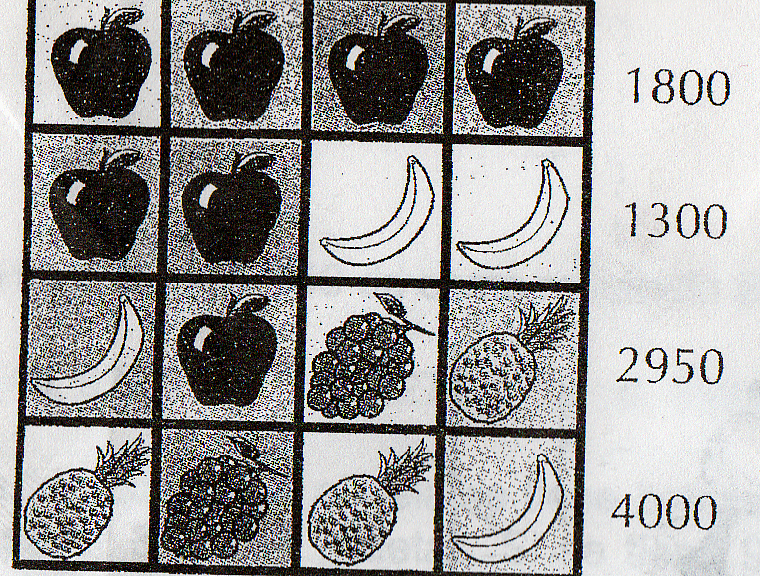
\includegraphics[scale=.2]{Images/frutas.png}}
\end{minipage}
\question \label{quest16}
¿Qu\'e precio tienen 6 manzanas, 3 bananos, 2 piñas y unas uvas?

\begin{oneparchoices}
\choice \$7000
\choice \$6500
\choice \$7500
\CorrectChoice \$7100
\end{oneparchoices}
\question ¿Cuánto debo pagar por 2 racimos de uvas, 3 piñas, 2 bananos y 1 manzana?

\begin{oneparchoices}
\choice \$4000
\choice \$6000
\CorrectChoice \$6950
\choice \$4950
\end{oneparchoices}
\question
¿Cuánto debo pagar por 3 manzanas, 3 bananos, 1 racimos de uvas y 1 piña?

\begin{oneparchoices}
\choice \$5000
\CorrectChoice \$4250
\choice \$4000
\choice \$2950
\end{oneparchoices}
\question ¿Qué precio tienen 8 manzanas?

\begin{oneparchoices}
\choice \$3000
\choice \$4000
\CorrectChoice \$3600
\choice \$1800
\end{oneparchoices}
\question \label{quest20}
¿Qu\'e precio tiene media docena de manzanas?

\begin{oneparchoices}
\choice \$2000
\choice \$1800
\choice \$3000
\CorrectChoice \$2700
\end{oneparchoices}
%\answerline
\end{questions}
%cuadro de puntajes
\end{document}